\subsection{Pipeline View}
\label{sec:pipeline}
Visual representation of the three stages (encoder, attention, classifier) model. In the proposed tool, we allow the model parameter to be updated to fix a prediction error (\textbf{T3}). The pipeline view, by showing the aggregated gradient distribution, we inform the user on the how different part of the model response to the optimization.

The optimization parameters is shown in (a), each of the stages is illustrated in (b), where the user can click on the parameter bar to enable or disable its update (the legend about its state is shown in (d) ). In (c), we select whether if we want to use current update setting as displayed or try all the configuration combination (i.e., each stage can be enabled or disabled).

\begin{figure}[htbp]
\centering
\vspace{-2mm}
 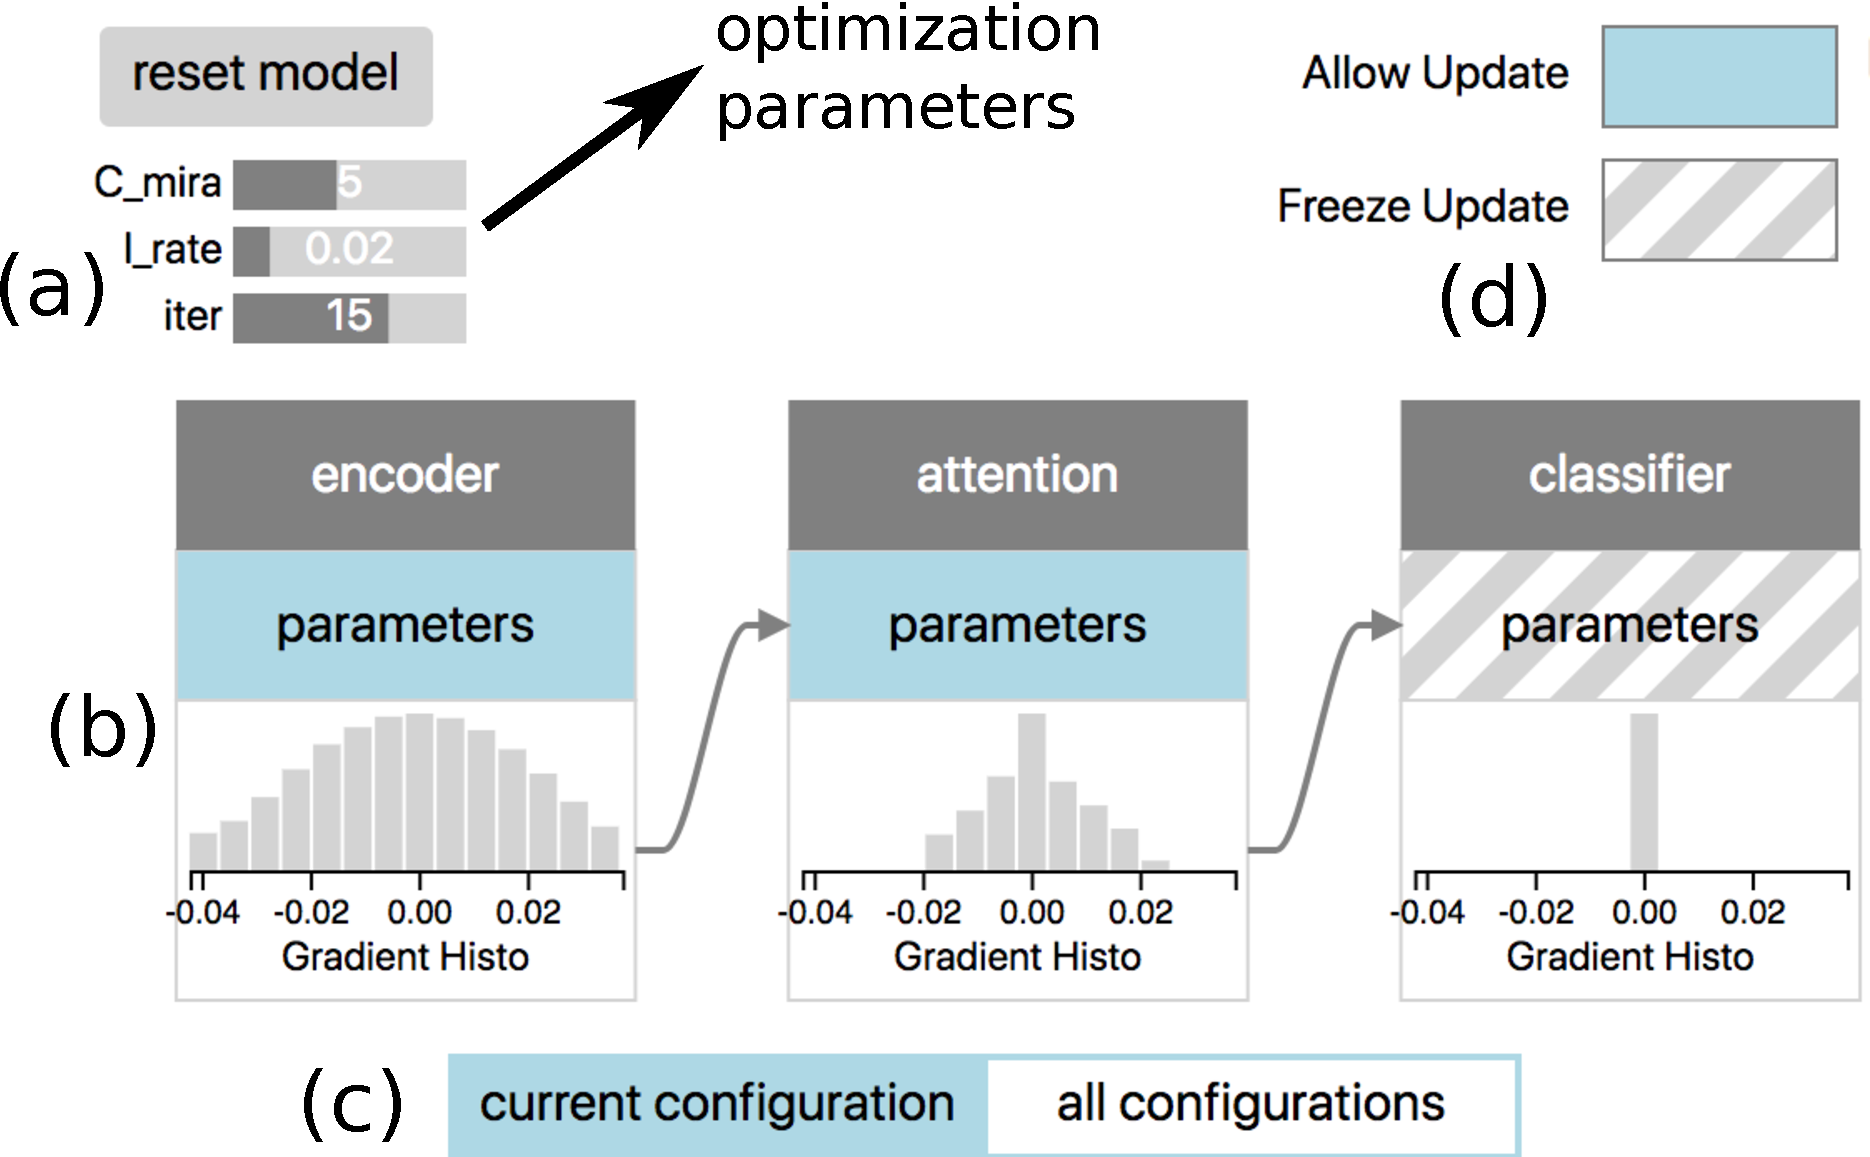
\includegraphics[width=1.0\linewidth]{pipelineView}
 \caption{
Visual representation of the three stages (encoder, attention, classifier) model. In the proposed tool, we allow the model parameter to be updated to fix a prediction error. The pipeline view, by showing the aggregated gradient distribution, inform the user about the how different part of the model response to the optimization.
%
The optimization parameters is shown in (a), each of the stages is illustrated in (b), where the user can click on the parameter bar to enable or disable its update (the legend about its state is shown in (d) ). In (c), we select whether if we want to use current update setting as display or try all the configuration combination (i.e., update for each stage can be enabled or disabled).
 }
\label{fig:pipelineView}
\end{figure}

% \textbf{Margin-Infused Relaxed Algorithm (MIRA)}
There are many way to update the model to correct a prediction. The simplest way to achieve it is applying standard back propagation that overfit to the example. However, without any constrain, the update step may alter the model in unexpected ways. \shusen{what is the benefit of using mira?}
Insetad, we adopted the \emph{Margin-infused relaxed algorithm (MIRA)}~\cite{CrammerSinger2003} update, where we regulate the optimization with the amount of change to the parameter. In the proposed tool, we define the mira loss as the following:
\begin{equation}
\mathrm{argmin}(  C J(w') + ||w' - w|| ),
\end{equation}
$J$ is the lost function for the model.
